%%%%%%%%%%%%%%%%%%%%%%%%%%%%%%%%%%%%%%%%%%%%%%%%%%%%%
%   Populações Estelares Simples
%%%%%%%%%%%%%%%%%%%%%%%%%%%%%%%%%%%%%%%%%%%%%%%%%%%%%

\chapter{Populações Estelares Simples}
%\addcontentsline{toc}{chapter}{Resultados}

\section{Uma Visão Geral}

Historicamente, a definição que ora empregamos de população estelar foi proposta inicialmente por um astrônomo e astrofísico dos Países Baixos, Jan Oort \cite{oort1926stars}, e posteriormente refinada por um astrônomo e astrofísico alemão, Walter Baade (Baade 1944), analisando os espectros das galáxias M31 e M32. Como conclusão, Baade percebeu que estes objetos consistem de uma mistura de dois tipos diferentes de estrelas, nomeados de população do tipo
I e população do tipo II. 

A primeira é constituída por estrelas jovens com idades menores que 7 × 10$^{9}$ anos, ricas em metais e que apresentam órbitas aproximadamente
circulares. Estrelas dessa classe são encontradas na estrutura de disco das galáxias espirais. Esse tipo de população apresenta diagrama cor-magnitude semelhante àqueles observados para aglomerados estelares abertos. Já o segundo tipo é constituído por estrelas com idades em torno de 10 × 10$^{9}$ anos ou da ordem da idade do Universo. São localizados preferencialmente no halo e bojo de galáxias espirais e galáxias elípticas. Podem ser pobres se estiverem localizadas no halo, ou ricas em metais
se estiverem presentes no bojo. Esse tipo de população estelar apresenta diagrama cor-magnitude semelhante aos observados para aglomerados globulares estelares.

Essa análise revela um resultado muito importante, pois permite caracterizar quais são os tipos de populações predominantes na classificação morfológica de Hubble (ver Figura 1). Nesse sentido, temos:

Galáxias Elípticas: consistem predominantemente de estrelas da População II;

Galáxias Lenticulares: seguem, geralmetne, o padrão da elípticas;

Galáxias Espirais: apresentam uma mistura de Populações I e II, as quais estão presentes nas regiões de disco e bojo/halo, respectivamente;

Galáxias Irregulares: apresentam em maior quantidade estrelas de População I.

No entanto, nada podemos dizer sobre as galáxias peculiares, pois não fazem parte dessa construção morfológica inicial. No entanto, como a nossa amostra espectral revelou tanto espectros de absorção quanto de emissão, é razoável supor que os dois tipos de populações estejam presentes ao final da síntese espectral. Na verdade, essa será a primeira discussão mais abrangente sobre as características populacionais nas galáxias com jatos presentes na Categoria 7 do Catálogo de Arp \& Madore.

Para o estudo da síntese espectral das galáxias selecionadas com jatos, iremos dividir as populações estelares usando como critério de diferenciação as respectivas idades. Nesse sentido, teremos:

Grupo 1. Extremamente jovens, com idades menores que 1 bilhão de anos, de modo que o "turn-off" (equivalente ao ponto de saída da sequência principal da população estelar correspondente), esteja próximo do tipo espectral A0. Em termos de massa (M$_\star$), corresponde a valores superiores a 2,4 M$_{\odot}$;

Grupo 2. Jovens, com idades entre 1 e 4 bilhões de anos, de modo que o "turn-off" da população correspondente esteja localizado entre os tipos A0 e F5, correspondendo ao intervalo de massa 2,4M$_{\odot}$ $<$ M$_{\star}$ $<$ 1,25M$_{\odot}$;

Grupo 3. Idade intermediária, com valores entre 4 e 10 bilhões de anos, de modo que o "turn-off" da população se localize entre os tipos F5 e G5, o que equivale a 1,25M$_{\odot}$ $<$ M$_{\star}$ $<$ 1,00M$_{\odot}$;

Grupo 4. Velhas, com idades entre 10 e 14,5 bilhões de anos, com o "turn-off" entre 0,90M$_{\odot}$ $<$ M$_{\star}$ $<$ 1,00M$_{\odot}$.

Aprendemos por exemplo, \cite{maciel1999amm} que as estrelas são, teoricamente, formadas de modo simultâneo a partir de um mesmo fragmento de nuvem de gás e poeira em contração, no qual apresenta uma composição química relativamente uniforme. Na verdade, consideramos que todas as estrelas formadas de diferentes massas iniciam suas evoluções simultaneamente na Sequência Principal de Idade Zero (ZAMS: Zero Age Mean Sequence). Assim, consideramos que a estrela começa seu tempo de vida sobe a Sequência Principal quando alcança a ZAMS. No que segue, usaremos o termo SP para a Sequência Principal.

Na literatura, uma "População Estelar Simples" (daqui para frente, SSP: Simple Stellar Population), consiste, basicamente, de um conjunto de estrelas que apresentam idades e metalicidades bem definidas. No entanto, para a construção de um modelo de uma SSP, é necessário o conhecimento de seus caminhos evolutivos para diferentes massas iniciais, composição química e função de massa inicial (IMF: Initial Mass Function), que é a função que expressa ou representa a distribuição numérica de estrelas por massa. Existe ainda a necessidade de termos o conhecimento das chamadas "Bases Estelares", "Trajetóras Evolutivas" e a "Função de Massa Inicial".  As bases representam grandes conjuntos de espectros que podem ser tanto empíricos como sintéticos. Possuem uma vasta abrangência em massa, idade e metalicidade, com diversos valores de temperatura e luminosidade, o que permite distribuir as estrelas de forma homogênea por todo o diagrama HR. No que tange as trajetórias evolutivas, conhecemos da teoria de evolução estelar que o tempo de vida de uma estrela isolada na SP e a respectiva trajetória no diagrama HR pós-SP, dependem, principalmente, da sua massa inicial de partida. Desse modo, quanto maior for a massa estelar, mais luminosa será a estrela na ZAMS, e mais rápida será a evolução. No que concerne a metalicidade, quanto menor, mais curto será o tempo evolutivo da estrela. 

\section{A Síntese de População Estelar}

A investigação proposta neste trabalho está pautada na síntese de população estelar das galáxias obtidas na literatura e aquelas observadas no OPD/LNA-MCTIC. De forma resumida, as diferentes técnicas existentes podem ser classificadas em duas linhas: (i) síntese de população estelar evolutiva e (ii) síntese de população estelar semi-empírica. O primeiro procura comparar os dados observados da galáxia com modelos que seguem a evolução de um sistema estelar inteiro, através da combinação de bibliotecas com caminhos evolutivos e espectros estelares. O segundo utiliza a informação contida nos espectros como descritos em Kenicutt \cite{kennicutt1998star}, como elementos de partida para se extrair as populações estelares existentes. Ambas técnicas apresentam vantagens e desvantagens, e diferenças em relação ao conjunto de observáveis que são sintetizados.

A comparação entre os dados observacionais e os modelos gerados é realizada em termos dos chamados “índices espectrais”, i.e., larguras equivalentes de linhas de absorção com emissão e cores (razões de fluxo em diferentes comprimentos de onda). Nesse sentido, os índices de Lick\footnote{O sistema de índices de Lick foi definido por \cite{faber}, e consta de um conjundo de características espectrais no intervalo óptico de 4000-6400 \AA.} \cite{trager1998old} e os definidos por \cite{bica1988A} estão entre os mais usados para fins de síntese espectral. Porém, embora contenham importantes informações espectrais, tais índices são, infelizmente, uma versão resumida do espectro real observado. Logo, é desejável que a comparação entre observação e modelo seja feita para todos os comprimentos de onda, pixel a pixel. Este trabalho se dedica a tal estudo, através da síntese de população estelar semi-empírica STARLIGHT (SEAGal - Semi-Empirical Analysis of Galaxies), Cid Fernandes et al. (\cite{cid2004star,fernandes2005semi,fernandes2007uncovering}).

Em décadas anteriores, a maneira empregada para se obter informações relativas às componentes das populações estelares nas galáxias, classificadas de acordo com o grupo definido acima, em muito jovens, x$_M${$_j$} 
(t \le 1 $\times$10$^8$ anos), jovens, x{$_J$} (1$\times$10{$^8$} < t \le 5$\times$10{$^8$} anos), de idades intermediárias x{$_I$}, (5$\times$10$^8$ < t \le 2$\times$10{$^9$} anos) e velhas x{$_O$} (t > 2$\times$10$^9$ anos), por exemplo, era realizada por meio da comparação direta de índices de linhas de absorção medidos no espectro integrado do sistema contra predições de grades de modelos de populações estelares simples, mais especificamente os índices espectrais de Lick \cite{trager1998old}. No entanto, uma maneira alternativa pela qual se pode obter informações acerca da mistura de populações estelares (e suas distribuições de composição química e idade), é feita através da análise “ponto a ponto” de todo o espectro integrado emitido pela galáxia, no caso da mesma não ter suas estrelas/subestruturas resolvidas angularmente. Porém, esse tipo de análise não é trivial, tendo em vista que não é possível identificar espectros estelares individuais a partir do espectro galáctico observado. O que temos, na verdade, é uma contribuição integrada do conjunto de estrelas presentes na galáxia (populações estelares que as compõem), sendo natural que cada população estelar apresente valores diferentes de idade e metalicidade.

\section{O Código STARLIGHT}

Adotamos para esta análise o código de síntese espectral STARLIGHT (SEAGal - Semi-Empirical Analysis of Galaxies), com o fim propósito de verificar como essas propriedades variam e dessa maneira inferir possíveis cenários de formação dessas galáxias peculiares, construindo pistas para caracterizar o jato observado nas mesmas. Trata-se, basicamente, de um código de síntese de populações estelares, desenvolvido em linguagem Fortran 77, que faz o ajuste de um espectro sintético, definido como M$_\lambda$, a um espectro observado de um sistema estelar, definido como O$_\lambda$.

Acrescentamos também análises de cinemática estelar para inferir sobre o estado dinâmico de cada galáxia e, deste modo, contribuir para obter um retrato mais completo acerca de um possível cenário de formação de cada galáxia da amostra. Aspectos geométricos como a inclinação na linha de visada, razão axial, excentricidade e elipticidade, quando possíveis, também serão abordados neste projeto. Todos os dados espectrais possíveis serão analisados à luz das informações fotométricas disponíveis na literatura. Os bancos de dados extragalácticos, NED/NASA-IPAC \url{ (https://ned.ipac.caltech.edu/)} e \url{HyperLeda (http://leda.univ-lyon1.fr/search.html)}, serão empregados no levantamento.

Basicamente, o método baseado no STARLIGHT consiste em modelar um espectro observado O$_\lambda$ usando uma combinação linear com coeficientes positivos dos elementos de uma base, que pode ser constituída tanto por observações (estrelas ou combinações de estrelas) ou por modelos teóricos (estrelas e populações estelares empíricas) de diferentes idades e metalicidades. Uma gaussiana é incluída para dar conta da cinemática e um termo para a extinção por poeira, de acordo com a equação:

 \begin{displaymath}
 \centering{
M\lambda=M_{\lambda  0}{[\sum_{j=1}^{N_{s}}}x_jT_j,\lambda r \lambda]\bigotimes G(v_s, \sigma_s)}
\end{displaymath}


\noindent onde M$_{\lambda}$ é o espectro sintético e M$_\lambda_0$ um fator de normalização, definido como o fluxo total de M$_\lambda$ no comprimento de onda $\lambda_0$;. T$_j,_\lambda$ representa o espectro da j-iésima componente da base, normalizado em $\lambda_0$; x$_j$ é a fração com que cada elemento T$_j,_\lambda$ da base contribui para o fluxo de M$_{\lambda}$; r$\lambda$ $\equiv$ 10$^{-0.4(A_\lambda-A_\lambda0)}$ leva em conta os efeitos de extinção por poeira. G(v$_s$,$\sigma_s$) é uma distribuição gaussiana de velocidades na linha de visada, centrada em v$_s$ e alargada por $\sigma_s$. O símbolo $\bigotimes$ expressa uma convolução.

O melhor ajuste definido é aquele que minimiza o x$^2$ entre o espectro observado (O$_\lambda$) e o modelo (M$_\lambda$):

 \begin{displaymath}
 \centering{
x^{2}=\sum_{\lambda}{}[(O_\lambda-M_\lambda)\omega_\lambda]^{2}}
\end{displaymath}

\noindent onde $\omega_\lambda$ é o inverso do ruí́do em O$_\lambda$. O algoritmo de Metropolis em conjunto com o “Simulated Annealing” \cite{mackay2003information} é empregado para evitar que o ajuste prenda-se por mínimos locais. Características espectrais não desejáveis no ajuste, ou por serem muito ruidosas ou por não estarem contempladas na base, podem ser mascaradas com a definição $\omega_\lambda$=0. Usaremos as trajetórias evolutivas de Padova 1994, recomendado por \cite{bruzual2003stellar}, com a função de massa inicial de Chabrier \cite{chabrier2003galactic}, entre 0,1 e 100 Msolar.

Os arquivos necessário para o código encontram-se disponíveis para download no site www.starlight.ufsc.br, com a devida versão para cada sistema operacional. De forma resumida, os arquivos de entrada necessários para utilizar este código são:

\begin{enumerate}

\item Espectro Observado - trata-se do espectro científico, calibrado em fluxo e em comprimento de onda de repouso. É importante ressaltar que o espectro esteja bem calibrado em fluxo, pois é a partir dessa precisão que o melhor ajuste de SSPs será obtido;

\item Máscara Espectral - trata-se de um arquivo para ignorar determinadas  regiões do espectro, como por exemplo, raios cósmicos, linhas telúricas, de emissão e extrações ruins que causam regiões com descontinuidade em fluxo;

\item Base Estelar - trata-se dos espectros estelares de SSPs a serem utilizados para ajustar o espectro sintético ao observado. 

\item Configuração - trata-se do arquivo que reúne as informações de partida (input) que serão carregadas pela código, incluindo, por exemplo, a normalização de contínuo, os limites para os parâmetros de cinemática e avermelhamento; 

\item Grade -  trata-se dos parâmetros das configurações definidas pelo usuário, e contém os espectros a serem ajustados, as base de SSPs, as máscaras, o intervalo em comprimento de onda que será adotado no ajuste, os limites de cinemática e lei de avermelhamento a ser usada: Cardelli, Calzetti ou Gordon.

\item Espectros de SSPs - trata-se dos espectros das populações estelares simples que serão utilizados pelo código STARLIGFHT.

\end{enumerate}

A Figura 6.1 ilustra alguns exemplos de espectros modelados com o código STARLIGTH, retirado do 'User Guide' disponível em http://www.starlight.ufsc.br/downloads/.

\begin{figure}[H]
	\centering	
    \caption{Saída do Código Starlight}
    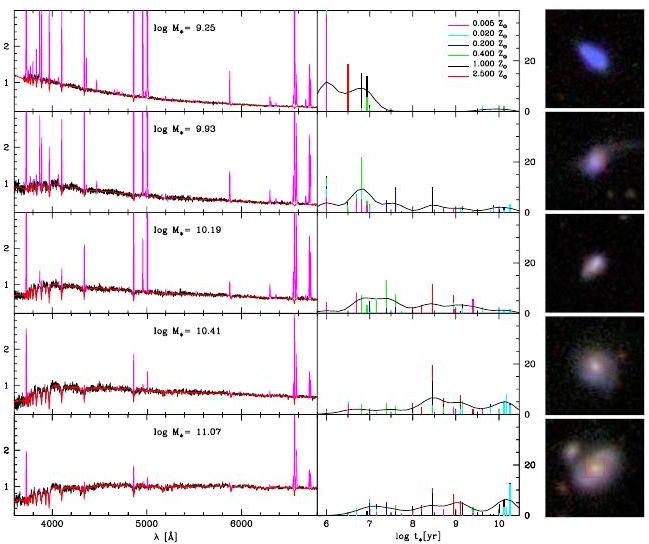
\includegraphics[width=1.0\textwidth]{figuras/starlight-ex.jpg}
   	\begin{center}
        \normalsize Fonte: \citeonline{Spectral fitting with STARLIGHT - 
Roberto Cid Fernandes. Disponível em http://www.starlight.ufsc.br/downloads/}\vskip 0.5cm \\Alguns exemplos de espectros ajustados. Lado esquerdo mostra o espectro observado (em preto) e o ajustado (em vermelho). Linhas verdes
marcam as regiões não consideradas no ajuste pois apresentam linhas de emissão. O painel do meio ilustra a fração da luz associada para cada uma das SSPs usadas no ajuste por ”bins” na escala de idade. O painel direito mostra imagens das galáxias analisadas extraídas da amostra presente no SDSS. 
    \end{center}
	\label{fig:sbmt-moses}
\end{figure}